\subsection{Assigning reviewers}

One of the primary reasons for using GitHub pull requests is to use its code review features.
We want both students and teachers to review code, with teachers explicitly having to approve a pull request for the assignment as a whole to be approved.

When assigning students we must make sure that no student is set to review an assignment they themselves have not yet completed.
Otherwise, we get a similar situation to the one mentioned in the previous challenge, where students have the option of plagiarising other students code.
Any implementation will have to make sure that students reviewing code should only review code they have already implemented.
A natural approach to this could be to have students only review code when the assignment deadline is passed.
At this point all students have gotten either a passing or failing grade, and QuickFeed can safely assign reviewers.

% No incentive for students to actually do code review when there is no penalty to refuse.

\subsection{Student feedback}

Another important feature is to have students receive automatic feedback on the code they write.
We envision that this feedback should come in the form of a score or grade, determined by tests run on the student's code.
Just as students currently receive feedback on an assignment as a whole, we want QuickFeed to do the same for tasks.

Currently, QuickFeed is only built around running tests on an assignment as a whole on the main branch.
To accommodate pull requests, QuickFeed would first need to be expanded so that it can run tests on other branches.
Secondly, QuickFeed will need the ability to run tests solely based on tasks.
The first accommodation is pretty straight forward, but the second one would require a rethink on how QuickFeed should approach the testing of code.

\subsection{Human Error}
% TODO: Can discuss these specifically in implementation part
Finally, we have to take into consideration the possibility that students may do things that we simply have not accounted for.

For example, they might delete issues that QuickFeed creates.
QuickFeed will then need to somehow recreate that issue, and restore a working state.

We will also have to account for students closing and possibly merging pull requests that are not yet approved by a teacher.
If this happens, QuickFeed must have the capacity to restore a working state for the task/assignment.

\subsection{Increased Complexity}

Introducing pull requests to students can prove challenging in itself.
Even though pull requests are not exactly a challenging feature to learn and use, it can still prove time consuming for certain students.
Even more so if students are already struggling with how to use git.
Having to swap between branches, making commits to them, and also knowing how to manage and create pull requests, are all things students will have to familiar with.
More time and effort from the teaching staff may therefore have to be dedicated to assisting students with issues they may have.

This is not an issue that can be explicitly solved.
Every teacher will have to decide themselves if the benefits outweigh the increased complexity when using tasks and pull request with their assignments.

\section{QuickFeed Expansion}
%% TODO: Move the contents from here to implementation.
Having simplified our approach in the previous section, we continue by looking at how we must expand QuickFeed to accommodate it.

\subsection{Tasks and GitHub Issues}
\label{sec:tasks_and_github_issues}

As a start, QuickFeed needs to support task markdown files in the \textit{tests} repository.
These task files will follow the standard format: \textit{task-*.md}.

\begin{figure}[ht]
    \centering
    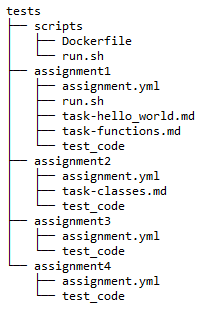
\includegraphics[scale=0.8]{photos/tests-repository-structure-tasks.PNG}
    \caption{Example of a tests repository with tasks}
    \label{fig:tests-repository-structure-tasks}
\end{figure}

As we see in the figure above, \textit{assignment1} and \textit{assignment2} both have tasks in them.

In essence we want these tasks to be represented as issues on all course group repositories.
This means that once a task is created by a teacher, and pushed to GitHub, the corresponding issues should be created on GitHub.
If a task is edited or deleted, QuickFeed must respectively either edit or delete the associated issue.
To manage the creation, deletion and editing of issues, QuickFeed's SCM API will be expanded to have such a capacity.

Beyond the ability to create, delete and edit issues, QuickFeed must be logically capable of determining when to perform these actions.
This means that QuickFeed will have to compare old tasks versus new ones, and then proceed accordingly.
We will therefore store representations of tasks in QuickFeed's internal database for this purpose.
Storing tasks also allows us to easily handle late enrolling groups, as we can use them to immediately create the required issues.

To edit issues, we will also need to internally store a reference to them in the database.

\subsection{Pull Requests}

The following questions are relevant for both this and the implementation part.

How do we listen to the webhook events that are relevant?
How do we single out the relevant events?
How should the pull requests be created?
How do we determine when to assign reviewers, when we do not have the ability to test based on tasks?
How do we ensure that reviewers are evenly distributed?
How do we ensure that reviewers are not assigned to their own repository?
What if a student pushes from a local branch that differs from a remote one?
What if an assignment is manually graded?

% To support pull requests, we need to expand

\subsection{Workflows}